% !TeX spellcheck = en_US
\addscenariosection{1}{Solo/Clash/Alliance Scenario}{Gold Rush}{\images/gold-mine.png}

\begin{multicols*}{2}

\textbf{Author:} farmaazon

\textbf{Source:} \href{https://discordapp.com/channels/740870068178649108/1344400556717768865/1344400556717768865}{Archon Studios Discord}

\textit{Your liege, engaged in costly wars in distant lands, has tasked you with extracting as much wealth as possible from this region. More importantly, you must find the legendary Grail to secure his ultimate victory.}

\subsection*{\MakeUppercase{Scenario Length}}

This Scenario is played over 13 Rounds.

\subsection*{\MakeUppercase{Player Setup}}

\textbf{Player Count:} 1, 2 or 4 (Alliance variant)

\textbf{Starting Resources:} 15 \svg{gold}, 3 \svg{building_materials}, 1 \svg{valuables}

\textbf{Starting Income:} 10 \svg{gold}, 0 \svg{building_materials}, 0 \svg{valuables}

\textbf{Starting Units:}
\begin{itemize}
  \item A Pack of chosen \bronze\ Units
  \item A Few cheapest \silver\ Units
\end{itemize}

\textbf{Town Buildings:} \bronze\ Dwelling, Citadel

\textbf{Map Tile Pool:} Each player takes 2 Far (II--III) Map Tiles.

\begin{center}
  {\transparent{0.2}
\includegraphics[width=0.7\linewidth, keepaspectratio]{\art/town_portal.png}}
\end{center}

\subsection*{\MakeUppercase{Map Setup}}

Take the following Map Tiles and arrange them as shown in the Scenario map layout ($P$ stands for the number of players):
\begin{itemize}
  \item $P$ × Starting (I) Map Tile
  \item $P$ × Far (II--III) Map Tile, each containing settlements
  \item $(P + 1)$ × Near (IV--V) Map Tile:  N1 and $P$ containing an Obelisk
  \item 2 × Center (VI--VII) Map Tile (C2 and \#C1\footnote{If you do not have the Tower expansion, you may use C1 instead of \#C1, with two changes: the \textit{Dragon Utopia} is treated as a Settlement, and the \textit{Warrior's Tomb} is protected by Neutral Units instead of the Shrine. All special rules related to \#C1 should then be applied to C1.})
\end{itemize}

\subsection*{\MakeUppercase{Additional Rules}}

\begin{table*}[b!]
  \hommtable[]{23}{
    \centering
    \begin{tabularx}{\linewidth}{p{0.25\linewidth}p{0.71\linewidth}}
      \darkcell{Tile and Location} & \darkcell{Additional Rules} \\
      \darkcell[1]{Obelisk}
      & \lightcell[1]{Choose one Minor Artifact from Resource Cards, or take 6 \svg{gold}} \\
      \darkcell[1]{N1 Witch Hut}
      & \lightcell[1]{Instead of standard effect, you may take \textit{Estates} Ability.} \\
      \darkcell[2]{\#C1 Warrior Tomb}
      & \lightcell[2]{Instead of \textbf{one} Artifact Search, you may choose Minor or Major Artifact from Resource Cards. The other Search must be from Artifact Deck.} \\
      \darkcell[1.3]{\#C1/C2 Shrine of Magic Incantation}
      & \lightcell[1.3]{Instead of searching for a Spell, you may take one \textit{View Air} Spell.} \\
      \darkcell[2]{\#C1 Settlement}
      & \lightcell[2]{Combat with Neutral Units cannot be skipped\textsuperscript{\hyperref[fn:combat]{*}}. The chosen settlement bonus is doubled\textsuperscript{\hyperref[fn:bonus]{**}}. Choose 5 (if you're first to Flag) or 2 (otherwise) artifacts from Resource Cards.} \\
      \darkcell[1.3]{C2 Grail}
      & \lightcell[1.3]{Combat with Neutral Units cannot be skipped\textsuperscript{\hyperref[fn:combat]{*}}. Take the Grail Token and lose all remaining \svgeven{movement-note}.} \\
    \end{tabularx}
    \medskip
  }
  \phantomsection
  \label{fn:combat}
  \footnotesize{\textsuperscript{*} Including Quick Combat. Bypassing without visiting the Field (such as with the \textit{Pathfinding} Ability) is still allowed.}

  \phantomsection
  \label{fn:bonus}
  \footnotesize{\textsuperscript{**} For example: if you choose increasing \svg{valuables} production, you increase it by two and get 2 \svg{valuables} if you are first player to Flag this settlement. If you choose reinforcement, you may reinforce two Units.}
\end{table*}

\begin{itemize}
  \item Before the game, remove all Cards that grant resources (including those with resource granting as one of the options) from their respective Decks, and form a \textbf{Resource Cards} pool. These Cards will be available at specific locations throughout the Scenario. If any of these Cards is removed from the game, it goes back to the pool.
  \item Lord Haart's starting \textit{Estates} Ability is replaced with \textit{Scouting}.
  \item At the start of certain Rounds, players must send a \textbf{tranche} to their lieges. The tranche value is expressed in \svg{gold}, but may be partially or entirely paid in other resources using these exchange rates: 1 \svg{building_materials} equals 2 \svg{gold} and 1 \svg{valuables} equals 4 \svg{gold}, with no change given. In Alliance mode, allied players collectively pay a single tranche. Any player or team unable to pay loses the game immediately.
  \item The difficulty of all Fields on the \#C1 Tile is lowered by one Level (effectively making it a ``V-VI'' Tile).
  \item Certain locations have special rules, typically allowing players to acquire \textbf{Resource Cards} -- refer to the table below.
  \item When defeating an enemy Main Hero, the victorious player may, instead of taking \mbox{5 \svg{gold}}, choose and take one Artifact from the opponent's Discard Pile.
  \item A Hero carrying the Grail Token is not protected by the \textit{Sanctuary} effect.
  \item If a Hero carrying the Grail Token surrenders or is defeated by an enemy Hero, they give the Token to the opponent.
  \item If a Hero carrying the Grail Token is defeated by a Neutral Army, the Grail Token is placed on the Field where the Hero was defeated. Any Hero visiting this Field takes the Token and loses all remaining~\svg{movement}.
\end{itemize}

\subsection*{\MakeUppercase{Victory Conditions}}

\begin{itemize}
  \item At the end of any Round, your Hero possesses the Grail Token and your team can afford all remaining \textbf{tranches}.
  \item In \textbf{PvP games}, if nobody wins after 13 Rounds, the winner is the player/team who is able to pay the highest \textbf{tranche} value with their remaining resources.
\end{itemize}

\vspace*{\fill}
\columnbreak

\subsection*{\MakeUppercase{Defeat Conditions}}

\begin{itemize}
  \item Fail to pay a required \textbf{tranche}.
  \item In \textbf{Solo play}: fail to meet the Victory Condition by the end of Round 13.
  \item In \textbf{PvP games}, if both players/teams cannot pay their \textbf{tranche} in the same Round, the player/team with the highest \textbf{tranche} value in remaining resources wins, with the Grail Token counting as 60~\svg{gold}.
\end{itemize}

\subsection*{\MakeUppercase{Timed Events}}

Players must pay tranches at the start of specific Rounds\footnote{The tranches are paid \textbf{after} other Round-beginning effects, including receiving resources or Astrologers Card}, as shown in the table below. After paying, \textbf{remove all Black Cubes} from every Windmill and Water Wheel on the map.

\medskip

\hommtablemulticol[]{14}{
  \centering
  \medskip
  \textbf{Tranches depending on the variant}\\
  \bigskip
  \begin{tabularx}{0.95\linewidth}{XXXX} \darkcell{Round} & \darkcell{Solo} & \darkcell{1v1} & \darkcell{2v2} \\
    \darkcell{\nth{4}}
    & \lightcell{20 \svg{gold}}
    & \lightcell{15 \svg{gold}}
    & \lightcell{30 \svg{gold}} \\
    \darkcell{\nth{8}}
    & \lightcell{50 \svg{gold}}
    & \lightcell{35 \svg{gold}}
    & \lightcell{70 \svg{gold}} \\
    \darkcell{\nth{12}}
    & \lightcell{80 \svg{gold}}
    & \lightcell{–}
    & \lightcell{–} \\
    \darkcell{\nth{13}}
    & \lightcell{–}
    & \lightcell{60 \svg{gold}}
    & \lightcell{120 \svg{gold}} \\
  \end{tabularx}
}

\vfill

\begin{center}
  {\transparent{0.2}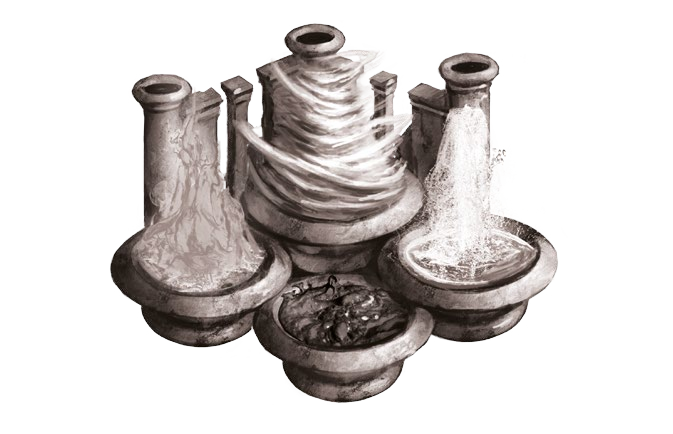
\includegraphics[width=\linewidth, keepaspectratio]{\art/elemental_conflux.png}}
\end{center}

\vfill


\begin{center}

\begin{tikzpicture}
  \node at (0.0, 0.0) {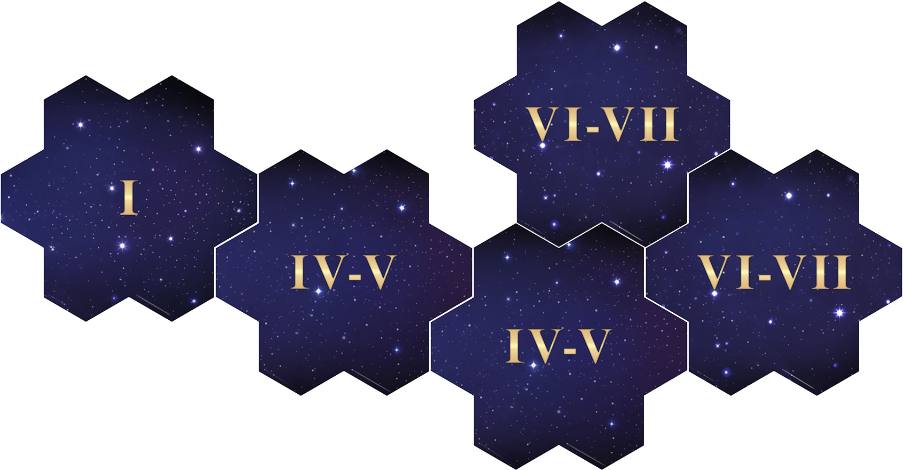
\includegraphics[width=0.6\linewidth]{\maps/gold_rush-solo.png}};
  \node at (1.0, -1.2) {\large{{\textbf{\textcolor{deepskyblue}{N1}}}}};
  \node at (1.27, 0.4) {\large{{\textbf{\textcolor{deepskyblue}{\#C1}}}}};
  \node at (1.56, 2.1) {\large{{\textbf{\textcolor{deepskyblue}{C2}}}}};
  \node at (0.0, -3.1) {\footnotesize{\textbf{SOLO VARIANT}}};
\end{tikzpicture}

\vfill

\begin{tikzpicture}
  \centering
  \node at (0.0, 0.0) {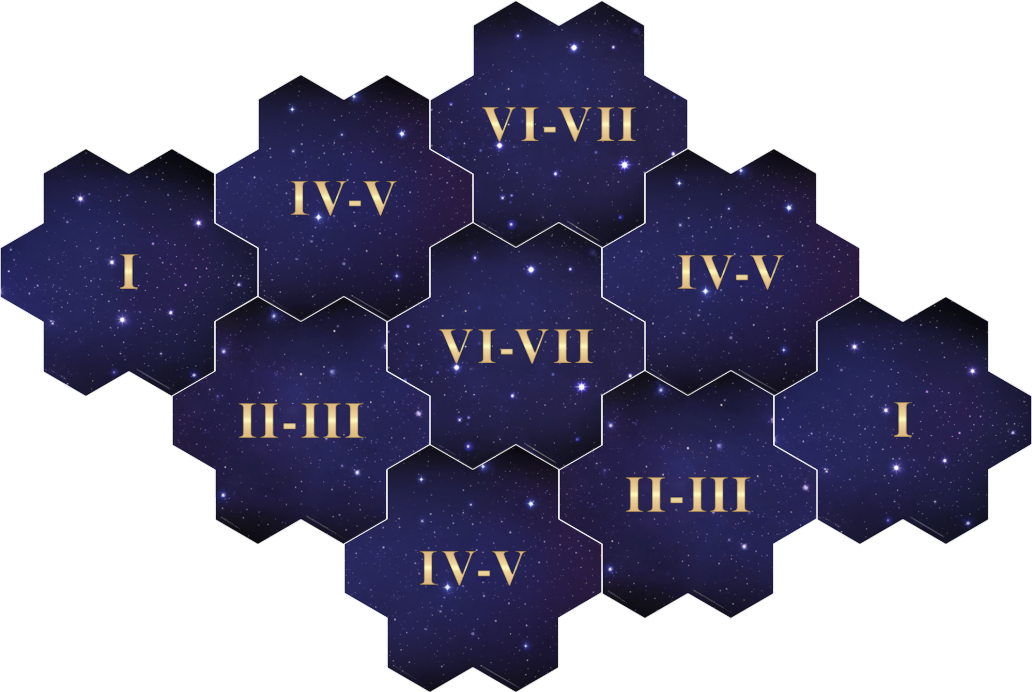
\includegraphics[width=0.92\linewidth]{\maps/gold_rush-1v1.png}};
  \node at (-0.25, -1.22) {\large{{\textbf{\textcolor{deepskyblue}{N1}}}}};
  \node at (0.0, 0.4) {\large{{\textbf{\textcolor{deepskyblue}{\#C1}}}}};
  \node at (0.35, 2.15) {\large{{\textbf{\textcolor{deepskyblue}{C2}}}}};
  \node at (0.0, -3.3) {\footnotesize{\textbf{1v1 VARIANT}}};
\end{tikzpicture}

\vfill

\begin{tikzpicture}
  \node at (0, 0) {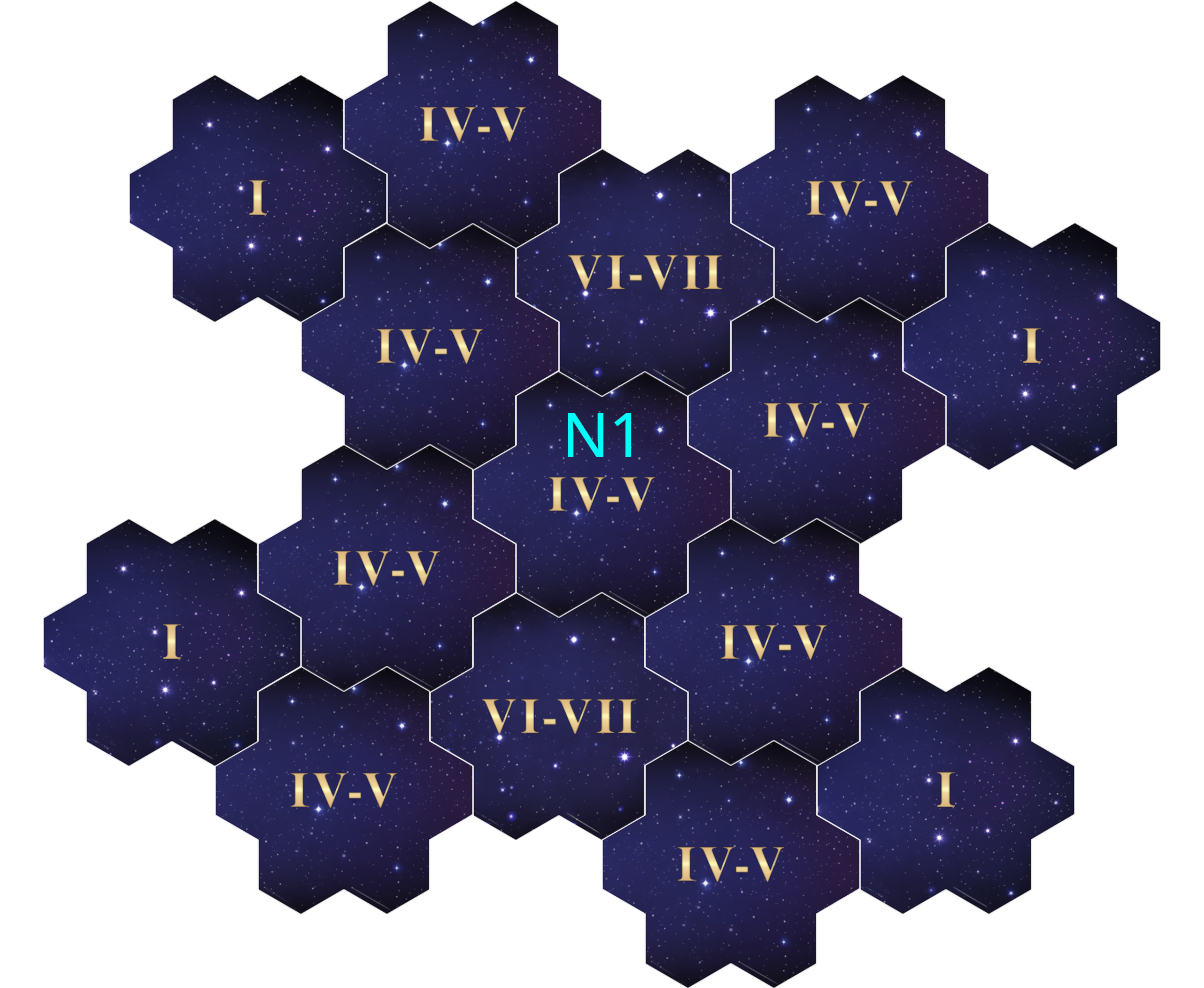
\includegraphics[width=\linewidth]{\maps/gold_rush-2v2.png}};
  \node at (0.03, 0.45) {\large{{\textbf{\textcolor{deepskyblue}{N1}}}}};
  \node at (0, -4.4) {\footnotesize{\textbf{2v2 VARIANT}}};
\end{tikzpicture}

\end{center}

\end{multicols*}
